\documentclass{article}
\let\vec\mathbf
\usepackage{graphicx}
\usepackage{amsmath}
\usepackage{gensymb}
\usepackage{float}
\graphicspath{{./documents/}{./figs}}
\begin{document}
\begin{enumerate}
\item During the lockdown period, many families got bored of watching $ TV $ all the time. Out of these families, 
 one family of 6 members decided to play a card game. 17 cards numbered 1, 2, 3, 4, . . . ,17 are put in a box 
 and mixed thorougly. One card is drawn by one member at random and other family members bet for the chances 
 of drawing the number either prime, odd or even etc.
		\begin{figure}[H]
			\centering
			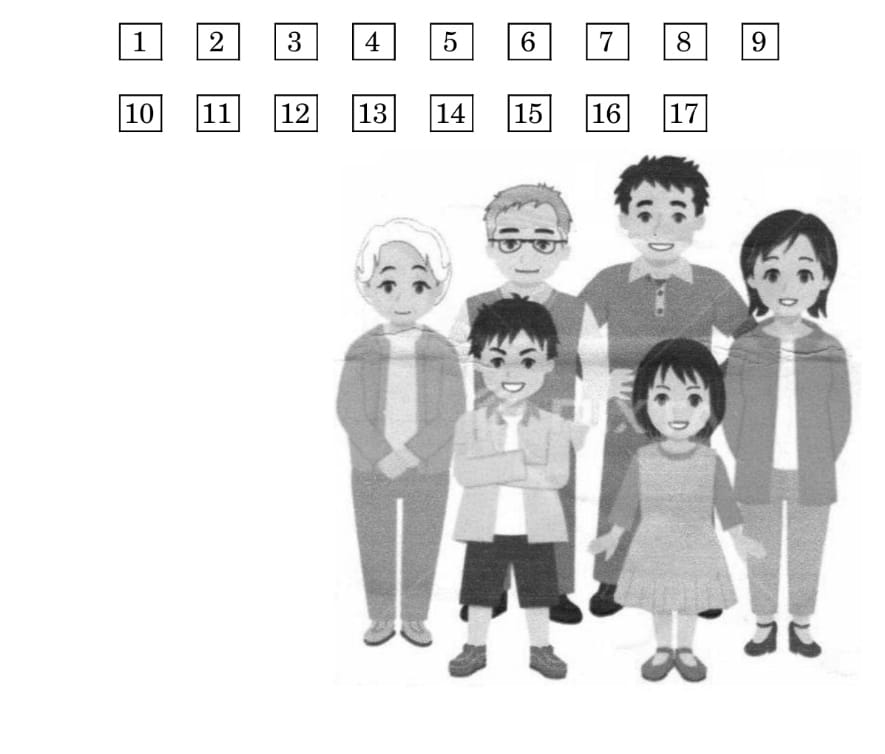
\includegraphics[width=\columnwidth]{figs/fig01.jpg}
			\caption{}
			\label{fig}
		\end{figure}
		Based on thee above, answer the following questions : 
		\begin{enumerate}
			\item The first member of the family draws a card at random and another member bets that 
				it is an even prime number. What is the probability of his winning the bet ?
				\begin{enumerate}
					\item $ \frac{2}{17} $
					\item $ \frac{3}{17} $
					\item $ \frac{1}{17} $
					\item $ \frac{4}{17} $
				\end{enumerate}
			\item The second member of the family draws a card at random and some other member bets 
				that it is an even number. What is the probability of his winning the bet ? 
				\begin{enumerate}
					\item $ \frac{7}{17} $
					\item $ \frac{8}{17} $
					\item $ \frac{9}{17} $
					\item $ \frac{10}{17} $
				\end{enumerate}
			\item What is the probability that the number on the card drawn at random is divisible 
				by 5 ?
				\begin{enumerate}
					\item $ \frac{5}{17} $
					\item $ \frac{4}{17} $
					\item $ \frac{3}{17} $
					\item $ \frac{2}{17} $
				\end{enumerate}
			\item What is the probability that the number on the card drawn at random is multiple 
				of 3 ? 
				\begin{enumerate}
					\item $ \frac{5}{17} $
					\item $ \frac{6}{17} $
					\item $ \frac{7}{17} $
					\item $ \frac{8}{17} $
				\end{enumerate}
			\item What is the probability that the number on the card is a factor of 9 ?
				\begin{enumerate}
					\item $ \frac{9}{17} $
					\item $ \frac{3}{17} $
					\item $ \frac{8}{17} $
					\item $ \frac{1}{17} $
				\end{enumerate}
		\end{enumerate}
	\item If the graph of a pair of lines $ x - 2y + 3 = 0 $ and $ 2x - 4y = 5 $ be drawn, that what type of 
		lines are drawn ? 
	\item
		\begin{enumerate}
			\item $ \vec{D} $ and $ \vec{E} $ are points on the sides $ CA $ and $ CB $ respectively 
				of a triangle $ ABC $, right-angled at $ \vec{C} $. \\
		        Prove that $ AE^2 + BD^2 =AB^2 + DE^2 $ 

			\item Diagonals of a trapezium $ ABCD $ with $ AB \parallel DC $ intersect each other at 
				the point $ \vec{O} $. If $ AB =2 CD $, find the ratio of the areas of triangles 
				$ AOB $ and $ COD $. 
		\end{enumerate}
	\item Write the steps of construction of drawing a line segment $ AB = 4.8 $ cm and finding a point 
		$ \vec{P} $ on it suchthat $ AP = \frac{1}{4} AB $. 
	\item Answer any $ four $ of the following questions : 
		\begin{enumerate}
		\item Given $ \Delta ABC ~ \Delta PQR $. If $ \frac{AB}{PQ} = \frac{1}{3} $, than 
			$ \frac{ar(\Delta ABC)}{ar(\Delta PQR)} $ is
			\begin{enumerate}
			\item $ \frac{1}{3} $
			\item 3
			\item $ \frac{2}{3} $
			\item $ \frac{1}{9} $
			\end{enumerate}
		\item The length of an altitude of n equilateral triangle of side 8 cm is
			\begin{enumerate}
				\item 4 cm
				\item $ 4\sqrt{3} $ cm
				\item $ \frac{8}{3} $ cm
				\item 12 cm
			\end{enumerate}
		\item In $ \Delta PQR, PQ = 6 \sqrt{3} $ cm, $ PR = 12 cm $ and $ QR = 6 cm $. The measure of 
			angle $ \vec{Q} $ is
			\begin{enumerate}
		\item $ 120{\degree} $
		\item $ 60{\degree} $
		\item $ 90{\degree} $
		\item $ 45{\degree} $
			\end{enumerate}
		\item If $ \Delta ABC ~ \Delta PQR $ and $ \angle{B} =46{\degree} $ and $ \angle{R} = 69{\degree}
			 $, then the measure of $ \angle{A} $ is
				\begin{enumerate}
					\item $ 65{\degree} $
					\item $ 111{\degree} $
					\item $ 44{\degree} $
					\item $ 115{\degree} $
				\end{enumerate}
			\item $ \vec{P} $ and $ \vec{Q} $ are the points on the sides $ AB $ and $ AC $ 
				respectively of a 
				$ \Delta ABC $ such that $ PQ \parallel BC $. If $ AP \parallel PB = 2 : 3 $ and 
				$ AQ = 4 cm $ then $ AC $ is equal to
				\begin{enumerate}
					\item 6 cm 
					\item 8 cm
					\item 10 cm
					\item 12 cm
				\end{enumerate}
		\end{enumerate}
	\item Answer any $ four $ of the following questions :
		\begin{enumerate}
			\item $ ABC $ and $ BDE $ are two equilateral triangles such that $ \vec{D} $ 
				is the mid-point of $ BC $. The ratio of the areas of the triangles 
				$ ABC $ and $ BDE $ is
				\begin{enumerate}
					\item 2 : 1
					\item 1 : 2
					\item 4 : 1
					\item 1 : 4
				\end{enumerate}
			\item In $ \Delta ABC, AB = 4 \sqrt{3} $ cm, $ AC = 8 cm $ and $ BC = 4 cm $. The angle 
				$ \vec{B} $ is
				\begin{enumerate}
					\item $ 120{\degree} $
					\item $ 90{\degree} $
					\item $ 60{\degree} $
					\item $ 45{\degree} $
				\end{enumerate}
			\item The perimeters of two similar triangles are 35 cm and 21 cm respectively. If one 
				side of the first triangle is 9 cm, then the corresponding side of the second 
				triangle is
				\begin{enumerate}
					\item 5.4 cm
					\item 4.5 cm
					\item 5.6 cm
					\item 15 cm
				\end{enumerate}
			\item In a $ \Delta ABC, \vec{D} $ and $ \vec{E} $ are points on the sides $ AB $ and 
				$ Ac $ respectively such that $ DE \parallel BC $ and $ AD : DB = 3 :1 $. 
				If $ AE = 3.3 cm $, then $ AC $ is equal to
				\begin{enumerate}
					\item 4 cm
					\item 1.1 cm 
					\item 4.4 cm
					\item 5.5 cm
				\end{enumerate}
			\item In the isosceles triangle $ ABC $, if $ AC = BC $ and $ AB^2 = 2AC^2 $, then $ 
				\angle{C} $ is equal to
				\begin{enumerate}
					\item $ 30{\degree} $
					\item $ 45{\degree} $
					\item $ 60{\degree} $
					\item $ 90{\degree} $
				\end{enumerate}
		\end{enumerate}




\end{enumerate}
\end{document}
